\section[Fundamental Concepts]{\hyperlink{toc}{Fundamental Concepts}}
\subsection{The Beginnings of Quantum Mechanics}
Here is a sample file for a chapter tex file

Here is an example for the equation:
\begin{equation}
    I_{\text{Wien}}(\lambda, T) \sim \frac{1}{\lambda^5}\exp(-\frac{1}{\lambda T}) % I(\lambda, T) = \frac{2hc^2}{\lambda^5}e^{-\frac{hc}{\lambda k_B T}}
\end{equation}
Looks great!
%\noident
In the following figure you can see a template for inserting images. Images are stored in a seperate folder in the Images. 
\begin{figure}[htbp]
    \centering
    \includegraphics[]{Images/fig-BBRspectra.pdf}
    \caption{This is the caption of the sample image!}
    \label{fig-BBRspectra}
\end{figure}


Also here is an example how to include a foot note!
In the above discussion, we have introduced Planck's constant. It has numerical value\footnote{which is the set/absolute (rather than measured) value of the Planck constant as per the 2018 redefinition of SI units.}.






\subsection{Kets, Bras, and Hilbert Space}
Here is an example of table!

\begin{table}[htbp]
    \centering\begin{tabular}{|c|c|}
        \hline Quantum states & $\ket{\psi} \in \H$ 
        \\ \hline Evolution & $i\hbar\pd{}{t}\ket{\psi} = H\ket{\psi}$
        \\ \hline Measurement & $\ket{\psi} \mapsto \frac{\Pi_j \ket{\psi}}{\sqrt{\bra{\psi}\Pi_j\ket{\psi}}} \quad p(j) = \bra{\psi}\Pi_j\ket{\psi}$
        \\ \hline
    \end{tabular}
    \caption{Axioms of quantum mechanics, concerning states, evolution, and measurement.}
    \label{table-QMaxioms}
\end{table}

Here are some examples for boxes

\begin{axiombox}{: Quantum states}\label{axiom-states}
    Quantum states $\ket{\psi}$ are vectors (also called ``kets'') in a complex Hilbert space $\H$.
\end{axiombox}



\begin{defbox}{: (Complex) Hilbert spaces}\label{def-Hilbertspaces}
    $\H$ is a (complex) Hilbert space if:
    \begin{enumerate}[(i)]
        \item $\H$ is a vector space over $\CC$
        \item $\H$ has an inner product
        \item $\H$ is complete (with respect to the metric induced by the norm induced by the inner product)\footnotemark - For the purposes of this course, this last point can be ignored.
    \end{enumerate}
\end{defbox}

\footnotetext{This is a technical qualification for the mathematicians in the crowd. An intuitive explanation for the curious; the inner product on a Hilbert spaces creates a notion of distance on the space. There are sequences (of vectors) that get closer together over time; completeness tells us that any such sequences (known as Cauchy sequences) must converge to a limit.}




\begin{defbox}{: Dual correspondence}\label{def-dualcorrespondence}
    To each vector space $\H$, there exists a dual vector space $\H^*$. There is a one-to-one correspondence\footnotemark between the kets $\ket{\psi} \in \H$ and the bras\footnotemark $\bra{\psi} \in \H^*$. We call this the \emph{dual correspondence}, and write it as follows:
    \begin{equation}
        \ket{\psi} \DC \bra{\psi}.
    \end{equation}
    It has the following properties:
    \begin{enumerate}[(i)]
        \item $\ket{\psi} + \ket{\phi} \DC \bra{\psi} + \bra{\phi}$
        \item $c\ket{\psi} \DC c^*\bra{\psi}$
    \end{enumerate}
    where the $*$ denotes complex conjugation.
\end{defbox}


\begin{propbox}{: Resolution of the identity}\label{thm-residentity}
    For all ONBs $\set{\ket{b_j}}_j$, the following relation holds:
    \begin{equation}
        \sum_j \dyad{b_j}{b_j} = \II
    \end{equation}
    where $\II$ is the identity operator on the Hilbert space.
\end{propbox}


\footnotetext{Formally, this follows from the Riesz Representation Theorem. But for the purposes of this course, we take this one-to-one correspondence as a postulate. Curious readers can find discussions/proofs of the theorem in any text on functional analysis, or mathematical quantum theory.}
\footnotetext{Given such names because $\braket{}{}$ is a bracket - bra-ket. Physicists remain unmatched in their sense of humour.}



\begin{figure}[htbp]
    \centering
    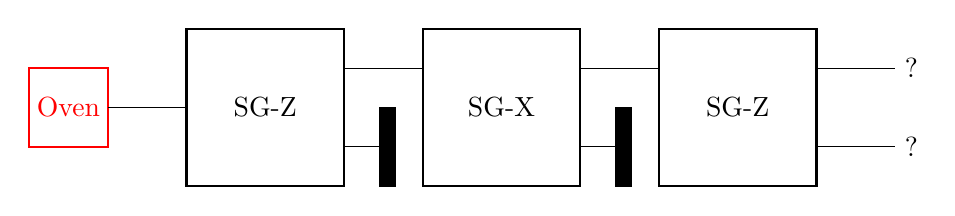
\begin{tikzpicture}
        \draw[red, thick] (0, 0) -- (1, 0) -- (1, 1) -- (0, 1) -- cycle;
        \node[red] at (0.5, 0.5) {Oven};
        \draw[] (1, 0.5) -- (2, 0.5);
        \draw[thick] (2, -0.5) -- (2, 1.5) -- (4, 1.5) -- (4, -0.5) -- cycle;
        \node[] at (3, 0.5) {SG-Z};
        \draw[] (4, 1) -- (5, 1);
        \draw[] (4, 0) -- (4.45, 0);
        \filldraw[fill = black, draw = black] (4.45, -0.5) -- (4.45, 0.5) -- (4.65, 0.5) -- (4.65, -0.5) -- cycle;
        \draw[thick] (5, -0.5) -- (5, 1.5) -- (7, 1.5) -- (7, -0.5) -- cycle;
        \node[] at (6, 0.5) {SG-X};
        \draw[] (7, 1) -- (8, 1);
        \draw[] (7, 0) -- (7.45, 0);
        \filldraw[fill = black, draw = black] (7.45, -0.5) -- (7.45, 0.5) -- (7.65, 0.5) -- (7.65, -0.5) -- cycle;
        \draw[thick] (8, -0.5) -- (8, 1.5) -- (10, 1.5) -- (10, -0.5) -- cycle;
        \node[] at (9, 0.5) {SG-Z};
        \draw[] (10, 1) -- (11, 1);
        \draw[] (10, 0) -- (11, 0);
        \node[right] at (11, 1) {?};
        \node[right] at (11, 0) {?};
    \end{tikzpicture}
   \caption{Here is an example figure using the latex utilities}
    \label{fig-SGsequential}
\end{figure}


Here is an example proof

\begin{proof}
    Recall that $\ket{\psi} = \sum_j \psi_j \ket{b_j}$ for any $\ket{\psi} \in \H$ and for any basis $\set{\ket{b_j}}_j$ of $\H$. Further, recall that $\psi_j = \braket{b_j}{\psi}$ if the basis is orthonormal. Hence we have that:
    \begin{equation}
        \ket{\psi} = \sum_j \braket{b_j}{\psi}\ket{b_j} = \sum_j \ket{b_j}\left(\braket{b_j}{\psi}\right) = \sum_j \left(\dyad{b_j}{b_j}\right)\ket{\psi} = \left(\sum_j \dyad{b_j}{b_j}\right)\ket{\psi}.
    \end{equation}
    Since the above relation holds for all $\ket{\psi}$, it follows then that $\sum_j\dyad{b_j}{b_j}$ is the identity as claimed.
\end{proof}

At this point in the course, the reader may be wondering what happened to quantum \emph{wavefunctions}\footnote{Though this nomenclature of ``wavefunction'' is arguably a misnomer; the Schr\"{o}dinger equation does not contain second order derivatives in time, as a wave equation would.}; the central objects of interest have instead been quantum states, without a wavefunction in sight. We now elucidate the connection between the two.

